\title{Solutions for Homework 5}
\author{Dr. Jordan Hanson - Whittier College Dept. of Physics and Astronomy}
\date{\today}
\documentclass[10pt]{article}
\usepackage[a4paper, total={18cm, 27cm}]{geometry}
\usepackage{graphicx}
\usepackage{amsmath}
\usepackage{tcolorbox}

\def\rcurs{{\mbox{$\resizebox{.16in}{.08in}{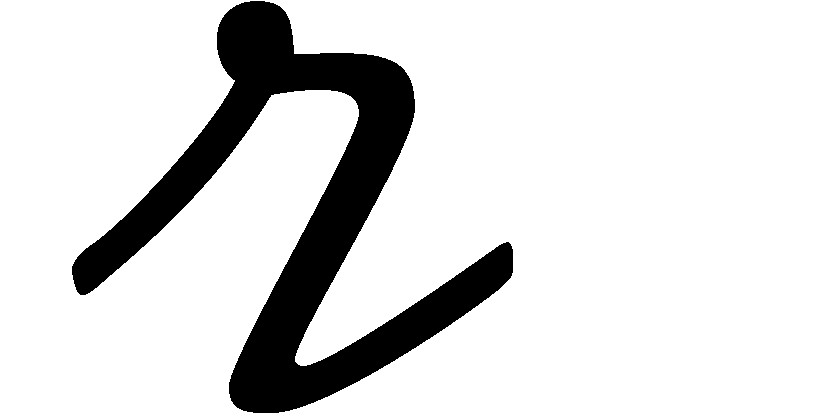
\includegraphics{ScriptR}}$}}}
\def\brcurs{{\mbox{$\resizebox{.16in}{.08in}{
\includegraphics{BoldR}}$}}}
\def\hrcurs{{\mbox{$\hat \rcurs$}}}

\begin{document}
\maketitle

\section{Problem 5.4}

\textit{Suppose that the magnetic field in some region has the form}

\begin{equation}
\mathbf{B} = kz \hat{\mathbf{x}}
\end{equation}
\noindent
\textit{(where k is a constant).  Find the force on a square loop (side a), lying in the $yz$-plane and centered at the origin, if it arries a current $I$, flowing counterclockwise, when you look down the $x$ axis.} \\ \\
Using $\mathbf{F} = I\mathbf{L} \times \mathbf{B}$, the Lorentz force for current in a magnetic field, we find 
\begin{equation}
\mathbf{F}_{\rm net} = Ika^2\hat{\mathbf{z}}
\end{equation}

\section{Problem 5.7}

\textit{For a configuration of charges and currents confined within a volume $\mathcal{V}$, show that}

\begin{equation}
\int \mathbf{J} d\tau = \frac{d\mathbf{p}}{dt}
\end{equation}
\noindent
\textit{where $\mathbf{p}$ is the total dipole moment. [Hint: evaluate $\int_\mathcal{V} \nabla \cdot (x \mathbf{J}) d\tau$].} \\ \\
\noindent
Folliwing the hint, keeping in mind that $\mathcal{V}$ contains all currents and charges (so none penetrate the surface $\mathcal{S}$ enclosing $\mathcal{V}$):

\begin{align}
\nabla \cdot (x \mathbf{J}) =& ~ x (\nabla \cdot \mathbf{J}) + \mathbf{J} \cdot (\nabla x) = -x \frac{\partial \rho}{\partial t} + J_x \\
\int_{\mathcal{V}} \nabla \cdot (x \mathbf{J}) d\tau =& \int_{\mathcal{V}} \left( -x \frac{\partial \rho}{\partial t} + J_x \right) d\tau \\
\int_{\mathcal{V}} \nabla \cdot (x \mathbf{J}) d\tau &= \oint_{\mathcal{S}} (x \mathbf{J}) \cdot d\mathbf{a} = 0 \\
\int_{\mathcal{V}} \left( -x \frac{\partial \rho}{\partial t} + J_x \right) d\tau &= 0 \\
\int_{\mathcal{V}} x \frac{\partial \rho}{\partial t} d\tau &= \int_{\mathcal{V}} J_x d\tau \\
\int_{\mathcal{V}} y \frac{\partial \rho}{\partial t} d\tau &= \int_{\mathcal{V}} J_y d\tau \\
\int_{\mathcal{V}} z \frac{\partial \rho}{\partial t} d\tau &= \int_{\mathcal{V}} J_z d\tau
\end{align}
\noindent
Combine the same arguement used for $x$ with the copies of it for $y$ and $z$.  Multiply by the corresponding unit vector on both sides of each each equation, and sum.  Then, switch the order of the time-derivative with the volume integration:

\begin{equation}
\int_\mathcal{V} \mathbf{J} d\tau = \frac{d}{dt}\int \mathbf{r} \rho d\tau = \frac{d\mathbf{p}}{dt}
\end{equation}
\noindent
In words, the volume integration of all current densities in a closed space is the time-derivative of the dipole moment of all charge.

\section{Problem 5.11}

\textit{Find the magnetic field at point $P$ on the axis of a tightly wound \textbf{solenoid} consisting of $n$ turns per unit length wrapped around a cylindrical tube of radius $a$ and carrying current $I$.  Express your answer in terms of $\theta_1$ and $\theta_2$ (Fig. 5.25).  Consider the turns to be essentially circular, and use the result of Ex. 5.6.  What is the field on the axis of an infinite solenoid?} \\ \\
The idea here is to sum the $\mathbf{B}$-field contributions from many circular loops of current at different distances.  Use Eq. 5.41 and Fig. 5.21 for a ring of width $dz$, with $I \rightarrow I n dz$:
\begin{equation}
B = \frac{\mu_0 n I}{2}\int \frac{a^2}{(a^2 + z^2)^{3/2}}dz
\end{equation}
Make the trigonometric substitution $z = a \cot(\theta)$ (Fig. 5.25).  The integral becomes
\begin{equation}
B = -\frac{\mu_0 n I}{2}\int_{\theta_1}^{\theta_2} \sin\theta d\theta = \frac{\mu_0 n I}{2}(\cos\theta_2 - \cos\theta_1)
\end{equation}
In the limit that the angles become 180 degrees and 0 degrees, for an infinite solenoid, the subtraction of cosines becomes 2, and we have $B = \mu_0 n I$, the formula for the constant field of a solenoid.

\section{Problem 5.12}

\textit{Use the result of Ex. 5.6 to calculate the magnetic field at the center of a uniformly charged spherical shell, of radius $R$ and total charge $Q$, spinning at constant angular velocity $\omega$.} \\ \\
Again, the concept is to add up many rings to build the object.  However, some amount of ``translation'' is required.  First, the radius of each ring (in terms of the zenith angle $\theta$) is $R\sin\theta$.  Second, the height $z$ above the center for each ring is $R\cos\theta$.  Each ring is meant to have a current $dI$, but $dI = K dl_{\perp} = K R d\theta$.  In this case, $K = \sigma v$, where $\sigma$ is the surface charge density: $\sigma = Q/(4\pi R^2)$.  The tangential velocity of a bit of charge around some ring at angle $\theta$ is $v = \omega R\sin\theta$.  Combining these translations together, we find
\begin{align}
dB &= \frac{\mu_0}{2R}\sin^2\theta dI \\
dI &= \frac{Q\omega}{4\pi}\sin\theta d\theta
\end{align}
Notice two things: if $\theta = \pi/2$, then that's charge moving around the equator, and $P$ is in the center of a ring of current, so $B \rightarrow \mu_0 I / (2 R)$, correctly.  Also, $dI$ is maximized at the equator, where it has the same \textit{period} but the largest \textit{radius}.  Putting the two pieces together and integrating $dB$ gives
\begin{equation}
\mathbf{B} = \frac{\mu_0 Q \omega}{6\pi R}\hat{\mathbf{z}}
\end{equation}
Several things make sense: the field does not exist of $\omega = 0$, or if $R \to \infty$.  The field is proportional to total charge because $Q\omega$ is like a current (units of C/s), so more charge gives a higher current and field.

\section{Problem 5.16}

\textit{Two long coaxial solenoids each carry current $I$, but in opposite directions (Fig. 5.42).  The inner solenoid (radius $a$) has $n_1$ turns per unit length, and the outer one (radius $b$) has $n_2$.  Find $\mathbf{B}$ in each of the three regions: (i) inside the inner solenoid, (ii) between them, and (iii) outside both.}
\begin{itemize}
\item (i) $\mathbf{B} = \mu_0 I (n_2 - n_1) \hat{\mathbf{z}}$
\item (ii) $\mathbf{B} = \mu_0 I n_2 \hat{\mathbf{z}}$
\item (iii) $\mathbf{B} = \mathbf{0}$
\end{itemize}
But isn't that interesting?  You could use this system to create a tunable field with precise control.  That is, depending on $n_1$, $n_2$, and different $I_1$ and $I_2$.  Problem 5.47 expands on this principle by introducing the \textbf{Helmholtz coil}, in which $\partial B/\partial z$ and $\partial^2 B/\partial z^2$ are both zero.

\section{Problem 5.19}

\textit{In calculating the current enclosed by an Amperian loop, one must, in general, evaluate an integral of the form}

\begin{equation}
I = \int_{\mathcal{S}} \mathbf{J} \cdot d\mathbf{a}
\end{equation}
\noindent
\textit{The trouble is, there are infinitely many surfaces that share the same boundary line.  Which one are we supposed to use?} \\ \\
We can show that it does not matter which surface is chosen, if $\nabla \cdot \mathbf{J} = 0$.  This means that $\mathbf{J}$ is a ``solenoidal'' field.  This means it can be written as the curl of some other vector field.  The curl theorem may then be used to change the surface integral to a line integral that does not depend on the surface it bounds.

\section{Problem 5.21}

\textit{Is Amp\`{e}re's law consistent with the general rule (Eq. 1.46) that divergence-of-curl is always zero?  Show that Amp\`{e}re's law cannot be valid, in general, outside magnetostatics.  Is there any such defect in the other three Maxwell equations?} \\ \\
Take the divergence of both sides of Amp\`{e}re's law:
\begin{equation}
\nabla \cdot (\nabla \times \mathbf{B}) = \mu_0 \nabla \cdot \mathbf{J}
\end{equation}
\noindent
The continuity equation states that
\begin{equation}
\nabla \cdot \mathbf{J} = -\frac{\partial \rho}{\partial t}
\end{equation}
We must, therefore, required that $\rho$ is constant, which is to say that currents are steady.  The other Maxwell's equations don't really have issues with second derivatives like this.

\section{Example 5.12 (Review)}

\textit{Find the vector potential of an infinite solenoid with $n$ turns per unit length, radius $R$, and current $I$.} \\ \\

\noindent

Remember the idea that the vector potential is usually parallel to currents:

\begin{equation}
\mathbf{A} = \frac{\mu_0}{4\pi} \int \frac{\mathbf{J}(\mathbf{r}')}{\rcurs} d\tau'
\end{equation}
\noindent
As long as the symmetry of the problem is showing us that the vector potential is parallel to current density, then the line integral of vector potential should be the easiest way to calculate it.  This procedure also assumes that we have some way of knowing the $\mathbf{B}$-field in advance.

\begin{equation}
\oint \mathbf{A} \cdot d\mathbf{l} = \int \mathbf{B} \cdot d\mathbf{a}
\end{equation}

\section{Problem 5.23}

\textit{Find the magnetic vector potential of a finite segment of straight wire carrying a current $I$.  [Put the wire on the $z$ axis, from $z_1$ to $z_2$, and use Eq. 5.66.]  Check that your answer is consistent with 5.37.} \\ \\
\noindent
Using Eq. 5.66, we find that
\begin{equation}
\mathbf{A} = \frac{\mu_0 I}{4\pi} \int \frac{d\mathbf{l}'}{\rcurs}
\end{equation}
\noindent
The best strategy is to simply look up the ensuing integral.  The result is
\begin{equation}
\mathbf{A} = \frac{\mu_0 I}{4\pi} \ln\left( \frac{z_2+\sqrt{z_2^2 + s^2}}{z_1+\sqrt{z_1^2 + s^2}} \right)\hat{\mathbf{z}}
\end{equation}
\noindent
To show that the correct $\mathbf{B}$-field corresponds to this vector potential, take the curl of it to reproduce Eq. 5.37.
\begin{equation}
\mathbf{B} = \nabla \times \mathbf{A} = -\frac{\partial A}{\partial s}\hat{\phi}
\end{equation}

\section{Problem 5.27}

\textit{Find the vector potential above and below the plane surface current in Ex. 5.8.}
\noindent
We already know that
\begin{equation}
\mathbf{B} = \pm \frac{\mu_0 K}{2}\hat{\mathbf{y}}
\end{equation}
\noindent
We also can see from the geometry of the problem that $\mathbf{A} = A(z)\hat{\mathbf{x}}$.  This implies, via the curl, that $\partial A/\partial z = \pm \mu_0 K/2$, so
\begin{equation}
\mathbf{A} = - \frac{\mu_0 K}{2}|z| \hat{\mathbf{x}}
\end{equation}
\end{document}

